\section{Results}

We present the results on \benchmarkname. Below, we detail the evaluation criteria, scaffold, and settings for reproducibility. We evaluate a suite of models, including frontier models, open-weight models, and models fine-tuned on SWE-bench-like trajectories (e.g. SWE-Smith).

\begin{table}[t]
\centering
\begin{minipage}{0.45\textwidth}
\centering
\begin{tabular}{@{}l c@{}}
\toprule
\textsc{Model} & \textsc{Resolve (\%)} \\
\midrule
\textsc{Claude Sonnet 4.5}                  & 43.6 \\
\textsc{Claude Sonnet 4} & 42.7 \\
\textsc{OpenAI GPT-5 (high)}               & 41.8 \\
\textsc{Claude Haiku 4.5}               & 39.5 \\
\textsc{Kimi K2 Instruct}               & 27.7 \\
\textsc{OpenAI GPT-OSS 120B} & 16.2 \\
\bottomrule
\end{tabular}
\caption{Model performance on the public set of \benchmarkname~(N=731). Models are evaluated using SWE-Agent \cite{yang2024sweagent}, without any ambiguity (e.g. we provide the augmented problem statement, requirements, interface).}
\label{table:results}
\end{minipage}
\hfill
\begin{minipage}{0.45\textwidth}
\centering
\begin{tabular}{@{}l c@{}}
\toprule
\textsc{Model} & \textsc{Resolve (\%)} \\
\midrule
\textsc{Claude Opus 4.1}     & 17.8 \\
\textsc{OpenAI GPT-5 (high)}      & 15.7 \\
\textsc{OpenAI GPT-5 (medium)}      & 14.9 \\
\textsc{Gemini 2.5 Pro Preview}     & 10.1 \\
\textsc{Claude Sonnet 4}   & 9.1  \\
\textsc{OpenAI GPT-4o}     & 3.6  \\
\bottomrule
\end{tabular}
\caption{Model performance on the commercial set of \benchmarkname~(N=276). Commercial problems are sourced from startup repositories, where each problem is augmented with an environment and relevant information.}
\label{tab:commerical-set}
\end{minipage}
\end{table}

\textbf{Scaffold.} We use the SWE-Agent \cite{yang2024sweagent} scaffold. We also explore another popular scaffold, Agentless \cite{xia2024agentless}. However, we find that Agentless has difficulty in multi-file editing, thus, produces low evaluation scores. We focus on SWE-Agent for our results.

\textbf{Evaluation settings.} All models use the latest versions as of September 18th, 2025. For open-source LLMs, we use vllm to host each model. Models are hosted on a single node, with 8 H100 Nvidia GPUs. We enable tool-use when possible, for open-weight models, we use syntax parsing to enable tool-use. Models have a maximum of 50 turns. We use the same prompt for all models, which is the default prompt from \cite{yang2024sweagent}. We use Opus 4.1 without extended thinking as reported by Anthropic in their own evaluation on SWE-Bench Verified.

\textbf{Issue Ambiguity.} Models are evaluated in the setting without any ambiguity -- that is, we include the problem statement, requirements and interface specification in the agent prompt. Here, models are evaluated on their ability to implement a given repair or patch after being given significant details (rather than their ability to resolve ambiguity).

\textbf{Evaluation sets.} Evaluations are done on the public set and commercial set. For all analysis, we use the public set to avoid potential leakage with the commercial set. Finally, we keep the private set held-out for future analysis.

\textbf{Results.} Table \ref{table:results} shows the results of various models on \benchmarkname. We report Pass@1 as the resolve rate. \textsc{Claude Sonnet 4.5} and \textsc{Claude Sonnet 4} achieve the highest resolve rates at 43.6\% and 42.7\% respectively, substantially outperforming smaller models. \textsc{OpenAI GPT-5 (high)} also achieves a 41.8\% resolve rate, while \textsc{Claude Haiku 4.5} demonstrates strong performance at 39.5\%. Earlier generation models like \textsc{Kimi K2 Instruct} and \textsc{OpenAI GPT-OSS 120B} show considerably lower performance at 27.7\% and 16.2\% respectively. There is also a significant performance gap between the public and commercial set, where the best models score less than 20\% in the commercial set, highlighting the difficulty of navigating enterprise codebases.
 
\begin{figure}[t]
\centering
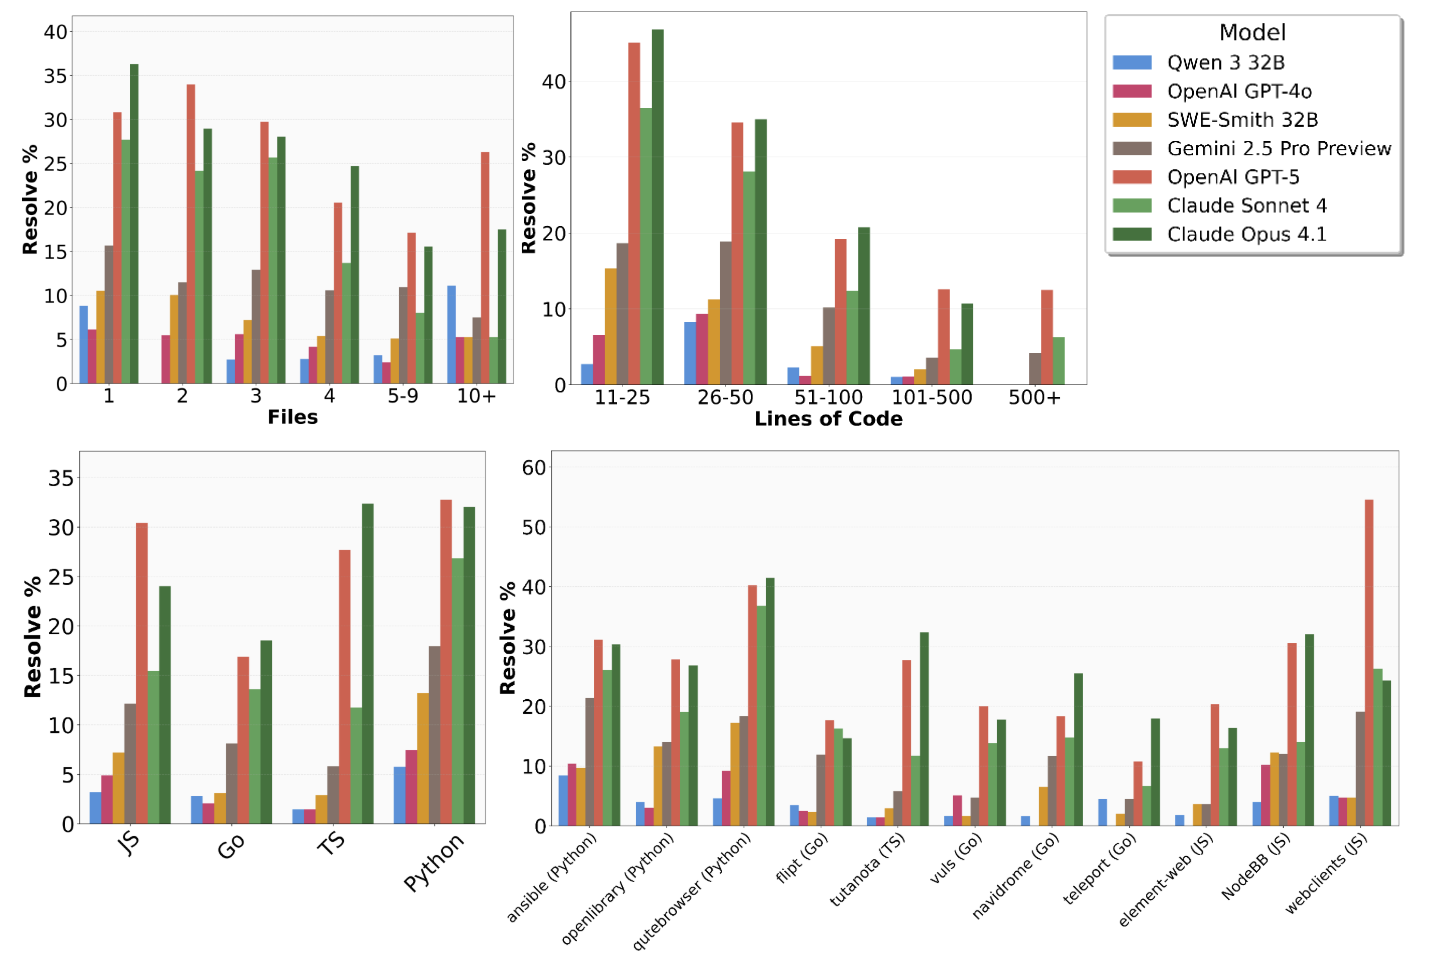
\includegraphics[width=\textwidth]{images/languages_and_repos.png}
\caption{Model performance varies across languages, and models current perform better at Python. Resolve rates across different repos in the public set of \benchmarkname. \benchmarkname~includes a variety of repos across different languages, with a similar number of problems per repo. Note that some categories, especially 10+ files and 500+ LOC, contain about 20-30 examples and thus have higher variance.}
\label{fig:languages_repos}
\end{figure}